\subsection{\cite{benoptical}}

\subsubsection{Staff Removal}

Staff removal in the application is attempted by generating performing an edge transform, then taking sections of a stave which contain five clear horizontal lines, connecting them up through the `unknown regions' and attempting to track the stave lines using these lines as a guide, removing pixels as it goes. In the case that no clear match is made between the guide line and stave line, the line is assumed straight, and pixels of a thickness which has already been seen are removed along it's length.

\subsubsection{Stem Detection}

For stem detection, since handwritten stems are unlikely to be perfectly straight, the authors use vertical projections combined with a high pass filter to establish likely stems, represented by peaks in the vertical projection.

A bounding box is then generated and the note is split into an upper and lower region, the upper and lower parts being used in note head and beam detection later.

\subsubsection{Note Head and Features Detection}

The author extracts the head position by way of a distances transform and then examining the density of the pixels (distance from the nearest black pixel) the results of which you can see graphically in \cref{fig:giloh-component-centre}. The authors also make several assumptions at this stage regarding the size of features (e.g. sharps are less than twice the stave space height) which enables them to separate notes from other components (clefs, accidentals etc).

\begin{figure}[H]
  \centering
  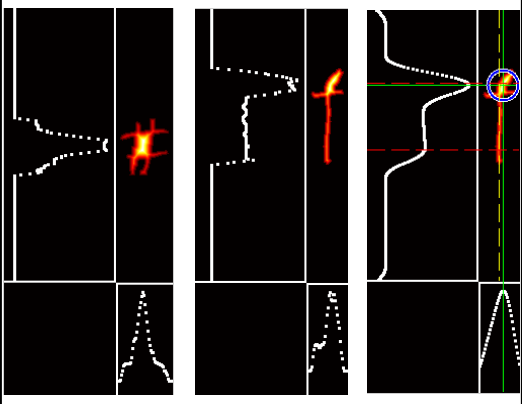
\includegraphics{gfx/prior-research/giloh-component-centre}
  \caption{Finding component centres, \parencite{benoptical}}
  \label{fig:giloh-component-centre}
\end{figure}
